
% tikz code as produced by R tikzdevice (script figmaxlik.r)
%% for figure figmaxlik used on line 966 from main.tex


% Created by tikzDevice
\begin{tikzpicture}[x=1pt,y=1pt, scale=0.4]
\draw[color=white,opacity=0] (0,0) rectangle (505.89,505.89);
\begin{scope}
\path[clip] ( 49.20, 61.20) rectangle (480.69,456.69);
\definecolor[named]{drawColor}{rgb}{0.50,0.27,0.14}
\definecolor[named]{drawColor}{rgb}{0.00,0.00,0.00}
\definecolor[named]{fillColor}{rgb}{0.00,0.00,0.00}

\draw[color=drawColor,line cap=round,line join=round,fill=fillColor,] ( 65.18,197.91) circle (  2.48);

\draw[color=drawColor,line cap=round,line join=round,fill=fillColor,] (137.82,271.15) circle (  2.48);

\draw[color=drawColor,line cap=round,line join=round,fill=fillColor,] (174.14,222.33) circle (  2.48);

\draw[color=drawColor,line cap=round,line join=round,fill=fillColor,] (246.78,319.98) circle (  2.48);

\draw[color=drawColor,line cap=round,line join=round,fill=fillColor,] (319.43,295.56) circle (  2.48);

\draw[color=drawColor,line cap=round,line join=round,fill=fillColor,] (355.75,393.22) circle (  2.48);

\draw[color=drawColor,line cap=round,line join=round,fill=fillColor,] (464.71,368.80) circle (  2.48);
\end{scope}
\begin{scope}
\path[clip] (  0.00,  0.00) rectangle (505.89,505.89);
\definecolor[named]{drawColor}{rgb}{0.50,0.27,0.14}
\definecolor[named]{drawColor}{rgb}{0.00,0.00,0.00}
\definecolor[named]{fillColor}{rgb}{1.00,1.00,1.00}

\draw[color=drawColor,line cap=round,line join=round,fill=fillColor,] (101.50, 61.20) -- (464.71, 61.20);

\draw[color=drawColor,line cap=round,line join=round,fill=fillColor,] (101.50, 61.20) -- (101.50, 55.20);

\draw[color=drawColor,line cap=round,line join=round,fill=fillColor,] (174.14, 61.20) -- (174.14, 55.20);

\draw[color=drawColor,line cap=round,line join=round,fill=fillColor,] (246.78, 61.20) -- (246.78, 55.20);

\draw[color=drawColor,line cap=round,line join=round,fill=fillColor,] (319.43, 61.20) -- (319.43, 55.20);

\draw[color=drawColor,line cap=round,line join=round,fill=fillColor,] (392.07, 61.20) -- (392.07, 55.20);

\draw[color=drawColor,line cap=round,line join=round,fill=fillColor,] (464.71, 61.20) -- (464.71, 55.20);

\node[color=drawColor,anchor=base,inner sep=0pt, outer sep=0pt, scale=  0.75] at (101.50, 37.20) {2};

\node[color=drawColor,anchor=base,inner sep=0pt, outer sep=0pt, scale=  0.75] at (174.14, 37.20) {4};

\node[color=drawColor,anchor=base,inner sep=0pt, outer sep=0pt, scale=  0.75] at (246.78, 37.20) {6};

\node[color=drawColor,anchor=base,inner sep=0pt, outer sep=0pt, scale=  0.75] at (319.43, 37.20) {8};

\node[color=drawColor,anchor=base,inner sep=0pt, outer sep=0pt, scale=  0.75] at (392.07, 37.20) {10};

\node[color=drawColor,anchor=base,inner sep=0pt, outer sep=0pt, scale=  0.75] at (464.71, 37.20) {12};

\draw[color=drawColor,line cap=round,line join=round,fill=fillColor,] ( 49.20, 75.85) -- ( 49.20,442.04);

\draw[color=drawColor,line cap=round,line join=round,fill=fillColor,] ( 49.20, 75.85) -- ( 43.20, 75.85);

\draw[color=drawColor,line cap=round,line join=round,fill=fillColor,] ( 49.20,197.91) -- ( 43.20,197.91);

\draw[color=drawColor,line cap=round,line join=round,fill=fillColor,] ( 49.20,319.98) -- ( 43.20,319.98);

\draw[color=drawColor,line cap=round,line join=round,fill=fillColor,] ( 49.20,442.04) -- ( 43.20,442.04);

\node[rotate= 90.00,color=drawColor,anchor=base,inner sep=0pt, outer sep=0pt, scale=  0.75] at ( 37.20, 75.85) {0};

\node[rotate= 90.00,color=drawColor,anchor=base,inner sep=0pt, outer sep=0pt, scale=  0.75] at ( 37.20,197.91) {5};

\node[rotate= 90.00,color=drawColor,anchor=base,inner sep=0pt, outer sep=0pt, scale=  0.75] at ( 37.20,319.98) {10};

\node[rotate= 90.00,color=drawColor,anchor=base,inner sep=0pt, outer sep=0pt, scale=  0.75] at ( 37.20,442.04) {15};

\draw[color=drawColor,line cap=round,line join=round,] ( 49.20,456.69) --
	( 49.20, 61.20) --
	(480.69, 61.20);
\end{scope}
\begin{scope}
\path[clip] (  0.00,  0.00) rectangle (505.89,505.89);
\definecolor[named]{drawColor}{rgb}{0.50,0.27,0.14}
\definecolor[named]{drawColor}{rgb}{0.00,0.00,0.00}

\node[color=drawColor,anchor=base,inner sep=0pt, outer sep=0pt, scale=  1.00] at (264.94, 13.20) {x};

\node[rotate= 90.00,color=drawColor,anchor=base,inner sep=0pt, outer sep=0pt, scale=  1.00] at ( 13.20,258.94) {y};
\end{scope}
\begin{scope}
\path[clip] ( 49.20, 61.20) rectangle (480.69,456.69);
\definecolor[named]{drawColor}{rgb}{0.50,0.27,0.14}
\definecolor[named]{drawColor}{rgb}{1.00,0.00,0.00}
\definecolor[named]{fillColor}{rgb}{1.00,1.00,1.00}

% y=0+bx
\only<2| handout:2>{\draw[color=drawColor,line cap=round,line join=round,fill=fillColor,line width=1pt] ( 49.20, 85.14) -- (480.69,282.36);}
% y=8+bx
\only<3| handout:3>{\draw[color=drawColor,line cap=round,line join=round,fill=fillColor,line width=1pt] ( 49.20,280.45) -- (480.69,477.67);}
% y=4.8+0.7x
\only<6| handout:6>{\draw[color=drawColor,line cap=round,line join=round,fill=fillColor,line width=1pt] ( 49.20,202.99) -- (480.69,400.20);}
% y=a+1.5x
\only<4| handout:4>{\draw[color=drawColor,line cap=round,line join=round,fill=fillColor,line width=1pt] ( 49.20,214.20) -- (338.51,505.89);}
% y=a+0.2x
\only<5| handout:5>{\draw[color=drawColor,line cap=round,line join=round,fill=fillColor,line width=1pt] ( 49.20,196.42) -- (480.69,254.43);}
\end{scope}
\end{tikzpicture}
